\chapter{Problemanalyse}
    \label{chapter:ProblemAnalysis}
    \section{Webseiten}
        Webseiten sind irrelevant für die Problemstellung.
        Es geht daraum den Inhalt aus einem CMS ins andere zu bekommen.
        Das hätte man auch machen können, ohne Webseiten zu betrachten.
        Auch dann, wenn Problemstellung CMS-Unabhängigkeit vorsieht,
        ist Webseiten Teil der Lösung (man hätte auch Abstraktionslayer mit Impl. für alle CMS schaffen können).
        Erst, wenn man sich fragt, wie man das erreichen kann, kommen Webseiten ins Spiel.

    \section{\imperia}
    \section{\wordpress}
    \section{Klassifizierung der Inhalte einer Webseite}
        \url{http://www.fernuni-hagen.de/KSW/portale/babw/service/}

        \begin{figure}
            \centering
            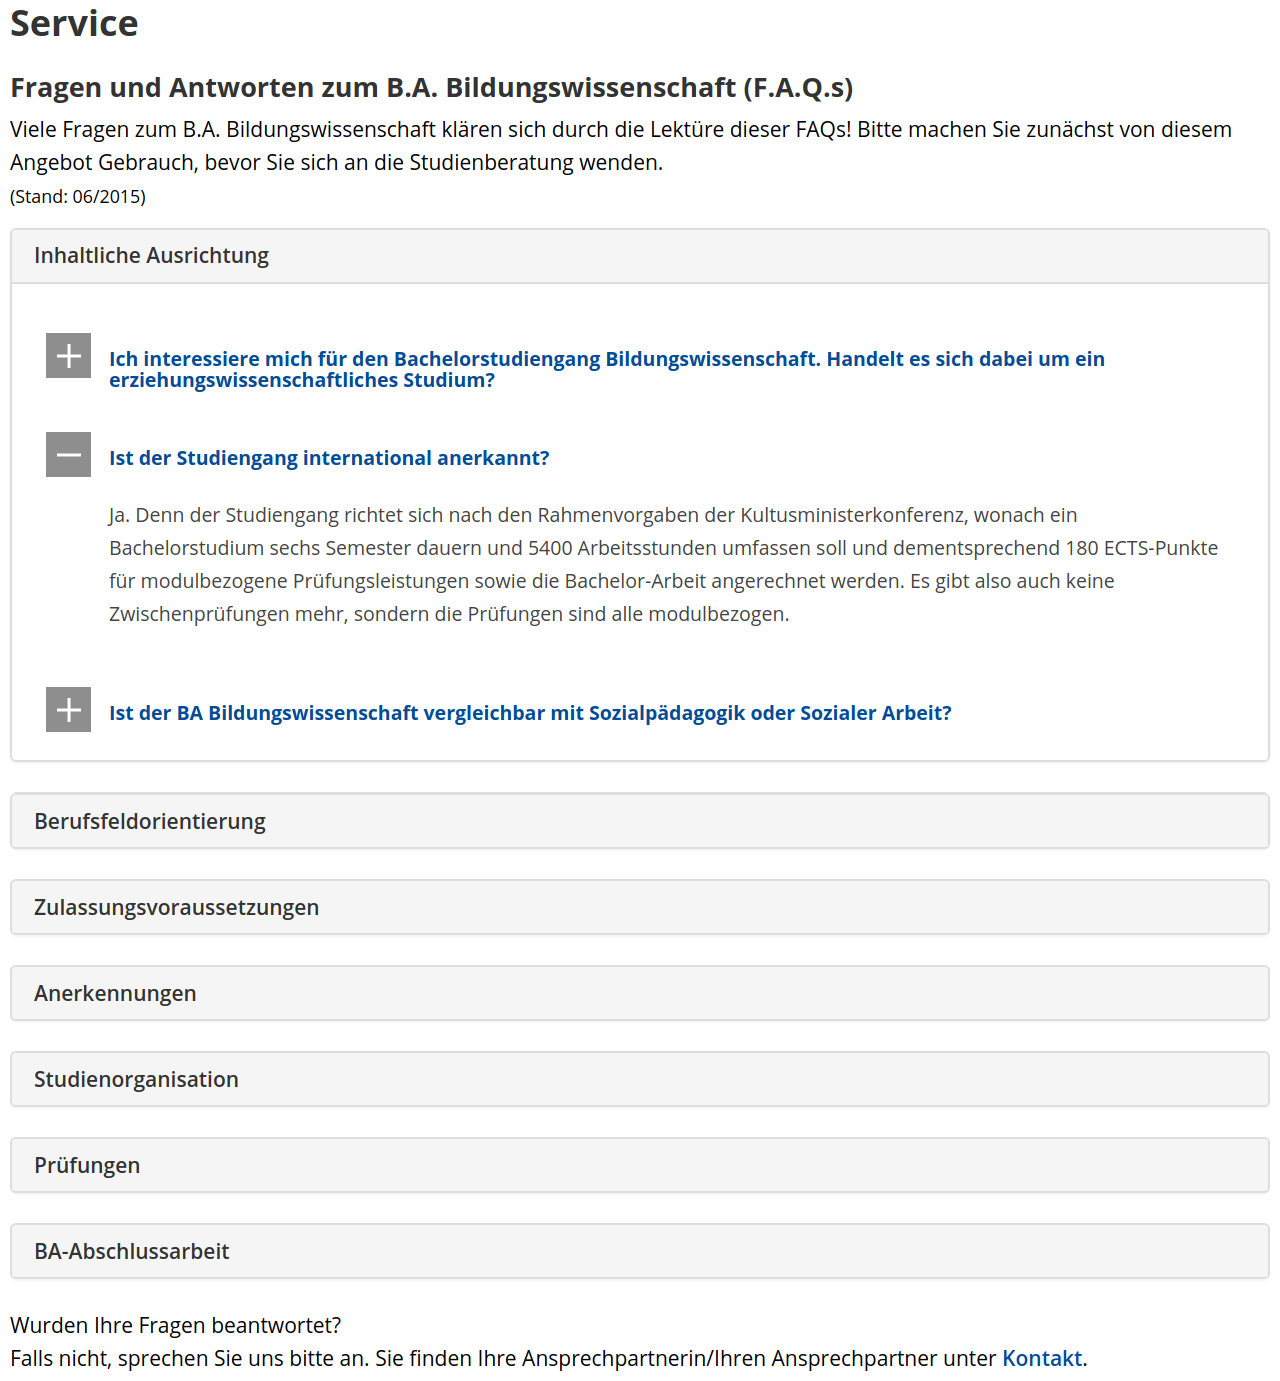
\includegraphics[width=\textwidth]{../resources/babw_service_faq.png}
            \caption{FAQ Seite des Studienportals B.A. Bildungswissenschaft}
            \label{image:BuildingBlocks}
        \end{figure}